\documentclass[10pt]{article}
\usepackage{longtable}
\usepackage{graphicx}
\usepackage{amssymb}
\usepackage{listings}
\usepackage[usenames]{color}
\usepackage[a4paper]{geometry}


\lstnewenvironment{c_code}[1][]
{\lstset{basicstyle=\small\ttfamily, columns=fullflexible,
keywordstyle=\bfseries, commentstyle=\color{blue},
language=C++, basicstyle=\small,showstringspaces=false, #1}}{}

 \newcommand{\qed}{\hfill \ensuremath{\Box}}
 \newenvironment{proof}{ \rm \begin{footnotesize}\noindent {\bf Proof}}{\qed \end{footnotesize}\\ \vspace{1cm} }
\cleardoublepage

\title{Documentation of  \\ReLIADiff. A C++ Software Package For Real Laplace
transform Inversion based on Algorithmic Differentiation
\footnote{Accompanying the paper in \cite{RELART}} }

\date{}


\begin{document}


\maketitle
\thispagestyle{empty}

\author{
\begin{center} LUISA D'AMORE\dag , ROSANNA CAMPAGNA\dag, VALERIA MELE\dag \\ ALMERICO MURLI\ddag \,  \

\end{center}}

{\dag\ University of Naples Federico II, Via Cintia,  Naples, Italy}


{\ddag\ CMCC -Lecce, Italy and SPACI}


\vspace{2cm}
\begin{center}
 {\large {\bf RELIADIFF SOFTWARE }}
\end{center}
\vspace{2cm}

\setlength{\parindent}{0in}
\newpage
\setcounter{page}{1}
\tableofcontents

\newpage

\section{Purpose} \label{sec:1}

RELIADIFF is a fully automatic software which computes the inverse $(f)$ of a Laplace transform function $(F)$ computable on the real axis.
It uses the software {\tt FADBAD/TADIFF} \cite{2} implementing the Algorithmic Differentiation. The mathematical background and general information about its performance are described in the accompanying paper \cite{RELART}.\\

RELIADIFF is a software package written in C++. To compile RELIADIFF and any software using RELIADIFF you need a C++ compiler.
If you do not have one:
\begin{itemize}
\item
On a Linux system we suggest to install GCC (GNU Compiler Collection,\\ {\tt http://www.gnu.org/software/gcc/gcc-4.6/}).
\item On a Windows system we suggest to install Bloodshed DEV-C++ IDE (v. 4.9.9.2,\\ {\tt http://www.bloodshed.net/dev/devcpp.html}).
\end{itemize}



\section{Outline of use}

The package consists essentially of the routine RELIADIFF. \\

\begin{figure}[!h]
\begin{flushright}
%[scale=0.6]
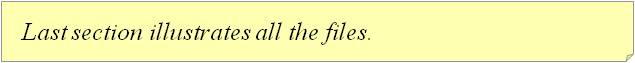
\includegraphics[scale=0.8]{rel1}
\end{flushright}
\end{figure}

To use the package, the user must provide
\begin{itemize}
\item a  context (such as a Main program) calling RELIADIFF;
\item a  function subprogram evaluating the transform $F(s)$, a double precision (in sense of {\tt TADIFF} \cite{2}) valued function  of  a double precision (in sense of {\tt TADIFF}) argument.
\end{itemize}

\begin{figure}[!h]
\begin{flushright}
%[scale=0.6]
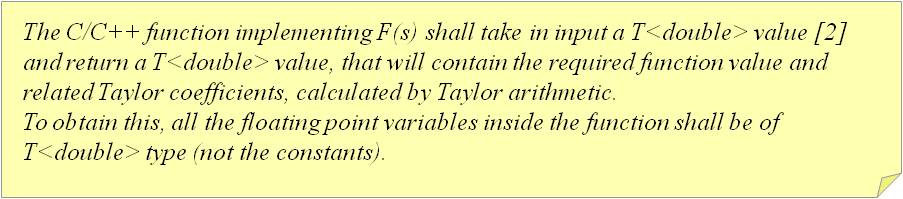
\includegraphics[scale=0.8]{rel2}
\end{flushright}
\end{figure}

Users have to include the header {\tt RELIADIFF.h}.\\

\begin{figure}[!h]
\begin{flushright}
%[scale=0.6]
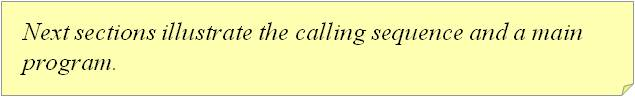
\includegraphics[scale=0.8]{rel3}
\end{flushright}
\end{figure}

The routine RELIADIFF needs as input
\begin{itemize}
\item
the function to invert $F$;
\item the value of $x\geq 0$ where the inverse function $f$ has to be computed;
\end{itemize}


User may tune the work of the software providing also (optionally):
\begin{itemize}
\item
the value of $sigma0$ (or an approximated value of it), the convergence abscissa of $F$;
\item a tolerance to the accuracy on $f(x)$;
\item the maximum number of series coefficients;
\item the singularity at zero of $F$;
\item the choice of printing all the used series expansion coefficients.
\end{itemize}


The software provides as output
\begin{itemize}
\item
the inverse Laplace function $f$ evaluated at the input point $x$;
\item the estimate of the absolute error on $f$;
\item the estimate of the relative error on $f$;

\begin{figure}[!h]
\begin{flushright}

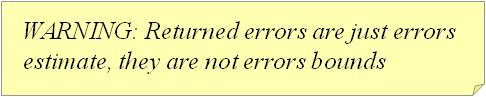
\includegraphics[scale=0.8]{rel4}
\end{flushright}
\end{figure}

\item some diagnostics parameters:
\begin{itemize}
\item the ``optimal'' number of series coefficients to use;
\item the number of series coefficients used to compute the ``optimal'' value;
\item a flag needed to interpret the work of the software.
\end{itemize}\end{itemize}

\begin{figure}[!h]
\begin{flushright}

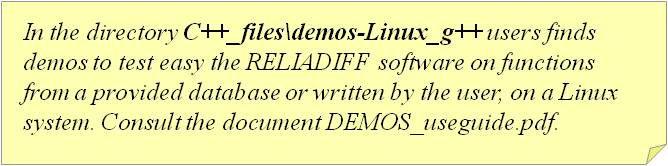
\includegraphics[scale=0.8]{rel5}
\end{flushright}
\end{figure}


\section{Specification}

\begin{center}
{\tt
\begin{tabular}{lll}
int RELIADIFF &(	&double x,         \\
		&&T<double> (*fz)(T<double>),\\
		&&char* szero,\\
		&&char* pcoeff,	\\
		&&char* sigma0, 	\\
		&&char* tol, 	\\
		&&char* nmax, 	\\
		&&double *ILf,	\\
		&&double *absesterr,\\
		&&double *relesterr, \\
		&&int *flag, 		\\
		&&int *nopt, 		\\
		&&int *ncalc, 		\\
	       &)&
\end{tabular}
}
\end{center}


\section{Arguments}

\subsection{Input Parameters}


 \begin{center}

\begin{longtable}{ll}
x  :	&	double precision\\
        & it contains value at which the Inverse Laplace Transform is required. \\
	&It has to be greater or  equal to zero.\\
&\\
fz :    &    	({\tt TADIFF}) double precision\footnote{See \cite{2} to know about the class {\tt T<double>}, that extends the C++ type {\tt double}.}  function pointer\\
	&it contains the name of the Laplace Transform function.\\
	&This function shall be written in C++\\
 \end{longtable}

\begin{figure}[!h]
\begin{flushright}

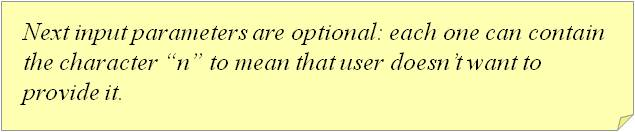
\includegraphics[scale=0.8]{rel6}
\end{flushright}
\end{figure}

\begin{longtable}{ll}
szero:	&	string\\
	&It contains\\
&\parbox{0.9\textwidth}{\begin{itemize}
\item   a parameter, interpreted as integer, specifying if the transform has a singularity at zero.\\
	IT CAN BE $0$ (there is nott) OR GREATER (there is).\end{itemize}}\\
&or\\
& \parbox{0.9\textwidth}{\begin{itemize}
\item   the character ``n'', to mean that the user does not want to provide it.\\
It will be posed to the default value ({\tt szero}$=0$).\end{itemize}}\\
&\\
pcoeff:	&	string\\
&it contains\\
&  \parbox{0.9\textwidth}{\begin{itemize}
\item  a parameter, interpreted as integer, specifying the printing or not of the coefficients in a file at the end of work.\\ IT CAN BE $0$ (do not print) OR GREATER (print).\end{itemize}}\\
&or\\
& \parbox{0.9\textwidth}{\begin{itemize}
\item
the character ``n'', specifying that the user does not want to provide it.\\
It will be posed to the default value ({\tt pcoeff}$=0$).\end{itemize}}\\
&\\
sigma0 :	& string\\
&It contains\\
&\parbox{0.9\textwidth}{\begin{itemize}
\item     the abscissa of convergence of $f$: it will be interpreted as double precision.
\item If it is less than zero, it will be posed to zero.\end{itemize}}\\
&or\\
&\parbox{0.9\textwidth}{\begin{itemize}
\item
the character ``n'', specifying that the user does not want to provide it.\\
It will be posed to the default value ({\tt sigma0}$=1$).\end{itemize}}\\
&\\
tol :     &     	string\\
&It contains\\
&\parbox{0.9\textwidth}{\begin{itemize}
\item     the required accuracy on $f$, interpreted as double precision;\\
\parbox{0.9\textwidth}{\begin{itemize}
\item if it is greater than $1$ it will be posed to the default value ($tol=10^{-3}$);\\
\item if it is less than the machine precision (single precision), it will be posed to the value of the machine precision.\end{itemize}}\end{itemize}}\\
&or\\
&\parbox{0.9\textwidth}{\begin{itemize}
\item
the character ``n'', specifying that the user does not want to provide it.\\
It will be posed to the default value ({\tt tol}$=10^{-3}$).\end{itemize}}\\
&\\
nmax:&	string\\
&It contains
\\
&\parbox{0.9\textwidth}{\begin{itemize}
\item  the maximum number of Laguerre series terms, interpreted as integer.\\
\parbox{0.9\textwidth}{\begin{itemize}
\item
if $nmax < 8$, it is posed equal to a default value ({\tt nmax }$= 2000$)\\
\item
if $nmax > MaxLength=5000$, it is posed at {\tt MaxLength}$ = 5000$.\end{itemize}}\end{itemize}}\\
&or\\
&\parbox{0.9\textwidth}{\begin{itemize}
\item
the character ``n'', specifying that the user does not want to provide it.\\
It will be posed equal to the default value ({\tt nmax}$ = 2000$).\end{itemize}}

 \end{longtable} \end{center}


\subsection{Output Parameters}

\begin{center}

\begin{longtable}{ll}
szero:	&	string \\
&It contains the value actually used by the software in computation, \\&it is interpreted as integer.\\
&\\
pcoeff:	&	string\\
&It contains the value actually used by the software in computation, \\&it is interpreted as integer.\\
&\\
sigma0 :&	 string\\
&It contains the value actually used by the software in computation, \\&it is interpreted as double precision.\\
&\\
tol :    &      	string\\
&It contains the value actually used by the software in computation, \\&it is interpreted as double precision.\\
&\\
nmax:	&	string\\
&It contains the value actually used by the software in computation, \\&it is interpreted as integer.\\
&\\
ILf :	&	double precision \\
&It contains the computed value of $f$ at $x$.\\
&\\
absesterr : 	&double precision\\
&It contains the estimate of the absolute error on $f$.\\
&\\
relesterr: &  	double precision \\
&It contains the estimate of the relative error on $f$.\\
&\\
flag: &       	integer  (DIAGNOSTIC) \\
&It contains an information on the obtained accuracy.\\
&\\
nopt:  &      	integer (DIAGNOSTIC) \\
&It contains the found ``optimal'' number of Laguerre series terms.\\
&\\
ncalc&	integer (DIAGNOSTIC)\\
&It contains the total number of terms calculated by the software \\
& to find the ``optimal'' one.

 \end{longtable} \end{center}

\subsection{Function Return Value}

\begin{center}

\begin{longtable}{ll}
Function return:&	integer.\\
&the function returns a diagnostic on the input data.\\
&if it is equal to $1$, it means that the routine ended without any output\\
& because the input $x$ was less than $0$.

 \end{longtable} \end{center}







\section{Calling sequence}

The variable declarations should be as follows:

\begin{center}
{\tt
\begin{tabular}{ll}
	double	&	x;	\\
	T<double>&	(*fz)(T<double>);\\
	char      &	szero[]; 	\\
	char	&	pcoeff[];	\\
	char	&	sigma0[];    \\
	char 	&	tol[];		\\
	char	&	nmax[]; \\
	double 	&ILf;		\\
	double	&	absesterr;\\
	double	&	relesterr;\\
	int	&	flag;	\\
	int	&	nopt;\\
	int	&	ncalc;	\\
	int	&	ierr;
\end{tabular}
}
\end{center}


The RELIADIFF call is then:

\begin{center}
\begin{verbatim}
 ierr= RELIADIFF (x, fz, pcoeff, sigma0, tol, nmax, szero, &ILf,
			&absesterr, &relesterr, &flag, &nopt, &ncalc);
\end{verbatim}
\end{center}




\section{An example of Calling Program}

A sample calling program to invert the function

$$F(z)=\frac{1}{z^4-a^4}, \qquad a=\frac{3}{5}$$

at the point $x=2.5$, without giving any optional input and printing results at screen is listed below.


\newgeometry{left=1cm,right=2cm}

\begin{c_code}

#include "RELIADIFF.h"
T<double> fzTest(T<double> z) {
	return 1./(pow(z,4)-pow(3./5.,4));
}
int main(int argc,char **argv){
/*RELIADIFF INPUT*/
          double 	x=2.5;		//Inverse Function evaluation point(s)
	T<double>	(*fz)(T<double>); 	//Function F Pointer

/*RELIADIFF OPTIONAL INPUT: we don't give any*/
	char        szero[10]="n";
	char		pcoeff[10]="n";
	char		sigma0[10]="n";
	char 		tol[10]="n";
	char		nmax[10]="n";

/*RELIADIFF OUTPUT*/
	double		absesterr;	//absolute error estimate
	double		relesterr;	//relative error estimate
	double 	ILf;		//Inverse Function f computed
	int		flag;	//diagnostics on the result
	int		nopt;	//diagnostics on the software work
	int		ncalc;	//diagnostics on the software work
	int		ierr;	//diagnostics on the software work

/*AUXILIARY VARIABLE*/
	char	name[20]="";

	fz = fzTest;

	/********************************** CALLING RELIADIFF *****************************************/
	ierr=RELIADIFF(x,fz,szero,pcoeff,sigma0,tol,nmax,&ILf,&absesterr,&relesterr,&flag,&nopt,&ncalc);
	/**********************************************************************************************/

	switch(ierr){
	case 1:
		printf("\nx=%f - RELIADIFF stopped: x<0.0!\n It must be x>=0\n\n",x);
		break;
	default:
		printf("Used Tolerance on accuracy: %e;\n",atof(tol));
		printf("Used abscissa of convergence on F: %e;\n",atof(sigma0));
		printf("Used maximum number of Laguerre series coefficients: %d;\n",atoi(nmax));
		printf("Singularity in zero: ");

		if(atoi(szero)) printf(" yes;\n");
		else printf(" no;\n");
		printf("Used Taylor coefficients printed: ");
		if(atoi(pcoeff)){
			sprintf(name,"coeff_x%.1f.txt",x);
			printf(" yes, they are in file %s;\n",name);
		}
		else printf(" no;\n");
		printf("\n                             TABLE\n");
		printf("-------------------------------------------------------\n");
		printf("|     x    |     f_comp     | estabserr | estrelerr |  Nopt |  Ncal |FLAG|\n");
		printf("-------------------------------------------------------\n");

		printf("| %4.2e | %14.8e | %9.3e | %9.3e | %5d | %5d | %2d |\n", x, ILf, absesterr, relesterr, nopt, ncalc, flag);
		break;
	} /*endswitch*/
	printf("\n***************************************************************************\n");
	printf("                 	               WARNING\n");
	printf("----Calculated errors are just errors estimate, they are not errors bounds---\n");
	printf("*****************************************************************************\n");
	printf("\n\nProgram terminated. Please press a key to exit.");	getchar();
	return 0;
}
/*END OF MAIN*/

\end{c_code}

\restoregeometry



\subsection{Output of the Calling Program Example}

Running the example program users will obtain at screen the following output.



\begin{verbatim}
Used Tolerance on accuracy: 1.000000e-03;
Used abscissa of convergence on F: 1.000000e+00;
Used maximum number of Laguerre series coefficients: 2000;
Singularity in zero:  no;
Used Taylor coefficients printed:  no;

			                  TABLE
---------------------------------------------------------------------------
|     x    |     f_comp     | estabserr | estrelerr |  Nopt |  Ncal |FLAG|
---------------------------------------------------------------------------
| 2.50e+00 | 2.61987232e+00 | 3.210e-04 | 1.225e-04 |    12 |    12 |  0 |

*******************************************************************************
                                    WARNING
----Calculated errors are just errors estimate, they are not errors bounds-----
*******************************************************************************

Program termineted. Please press a key to exit.

\end{verbatim}


\section{How To run the Calling Program Example}

{\bf {\em The package directory is C++$\_$files/src and it contains the above Calling Program Example, and two directory to execute it on either a Linux or a Windows system.
}}

\begin{figure}[!h]
\begin{flushright}
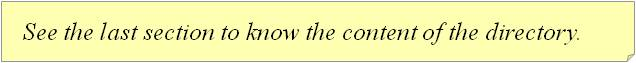
\includegraphics[scale=0.8]{rel9}
\end{flushright}
\end{figure}

\subsection{On a Linux system, with a g++ compiler installed}


To easy obtain the previous output, user can execute the script\\
{\bf CallingProgramExecution-Linux$\_$g++/compiling$\_$a$\_$CallingProgram.sh}.\\
The script will
\begin{enumerate}
\item create a RELIADIFF library with the command make
\item compile the calling program,
\item link it to the RELIADIFF library
\item execute the executable file.
\end{enumerate}


\subsection{On a Windows system, with Bloodshed DEV-C++ IDE v. 4.9.9.2 installed}


(To download DEV, visit: {\tt  http://www.bloodshed.net/dev/devcpp.html}\footnote{Bloodshed Dev-C++ is a full-featured Integrated Development Environment (IDE) for the C/C++ programming language. It uses Mingw port of GCC (GNU Compiler Collection) as its compiler. It creates native Win32 executables, either console or GUI. Dev-C++ can also be used in combination with Cygwin.\\
Dev-C++ is Free Software (also referred as Open Source), and is written in Delphi [{\tt http://www.bloodshed.net/dev/}].})\\

To easy obtain the previous output, user can open the file\\
{\bf\small CallingProgramExecution-Windows$\_$DevC++5/ExampleCallingRELIADIFFproject.dev}\\
then click on Execute $\to$ Compile $\&$ Run.\\
It will create in its directory the following files:

\begin{itemize}
\item {\tt ExampleCallingRELIADIFFproject.layout}
\item {\tt ExampleCallingRELIADIFFproject.exe} (executable)
\item {\tt Makefile.win}
\item {\tt phi.o}
\item {\tt RELIADIFF.o}
\item {\tt SimpleCallingProgramExample.o}
\end{itemize}

\section{Analysis of  the Diagnostic parameters}


\begin{description}

\item $flag$: it is about the obtained accuracy.

\begin{itemize}
\item[] $flag =0$: corresponds to:
\begin{itemize}
\item $absesterr < tol$
\item $relesterr < tol$
\end{itemize}

Both the absolute and the relative error estimates are smaller than tolerance, so the software fully satisfies the required accuracy. \\
This means that the software can obtain more accurate results if user requires a smaller value for the tolerance.

 \item[] $flag =1$: corresponds to the case of output:
\begin{itemize}
\item
$absesterr$ is the minimum obtained value, but greater than tolerance.
\item $relesterr$ is the minimum obtained value, but greater than tolerance.
\end{itemize}
This means that within $nmax$ terms of the series expansion, the algorithm cannot satisfy the required accuracy. So, it provides the numerical result within the maximum attainable accuracy with no more than $nmax$ terms, and $nopt$ will be the  number of terms  at which such minimum is reached (eventually different from $ncalc$, that is the total number of calculated coefficients). \\
Moreover, this means that the series seems to converge too slowly or to diverge.\\
So, user can try to obtain a  result more accurate tuning some of the optional parameters: $sinf$, $sigma0$, $nmax$.\\
User is also invited  to verify if the Laplace transform function satisfies algorithm's requirements.

 \item[] $flag =2$: corresponds to the case of output:
\begin{itemize}
\item $absesterr < tol$.
\item $relesterr$ is the minimum obtained value, but greater than tolerance.
\end{itemize}
            Only the absolute error estimate is smaller than the user's required accuracy. \\
This means that within $nmax$ terms of the series expansion, the algorithm cannot satisfy the required accuracy. So, it provides the numerical result within the maximum attainable accuracy with no more than $nmax$ terms, and $nopt$ will be the  number of terms  at which such minimum is reached (eventually different from $ncalc$, that is the total number of calculated coefficients). \\
Moreover, this means that the inverse function $f$ rapidly decreases towards zero.\\
User can try to obtain a  result more accurate tuning some of the optional parameters: $sinf$, $sigma0$, $nmax$.

\item[] $flag =3$: corresponds to the case of output:
\begin{itemize}
\item $absesterr$ is the minimum obtained value, but greater than tolerance.
\item $relesterr < tol$.
\end{itemize}
 Only the relative error estimate is smaller than the user's required accuracy.\\
This means that within $nmax$ terms of the series expansion, the algorithm can   satisfy the required accuracy, but not for the relative error. This means also that the inverse function $f$ increases rapidly.

\item  $RETURN\,\, VALUE$:

\begin{itemize}
\item[] $=1$: $x<0$, the run stopped without working.
\item[] $=0$: RELIADIFF worked properly.
\end{itemize}

\item  $ncalc / nopt$:
\begin{itemize}
\item	$ncalc$ is the maximum number of terms of the Laguerre series expansion calculated by the algorithm.
\item	$nopt$ is the number of terms of the Laguerre series expansion that gives the numerical result within the maximum attainable accuracy, less or equal to $nmax$ (the required maximum number of terms).
\end{itemize}
You can find one of three cases:
\begin{itemize}
\item[a.] $nopt=ncalc<nmax$
\begin{itemize}
\item[] The computed  value of the inverse Laplace function agrees with the true one within $\log(tol)$ significant and decimal digits. This value is obtained calculating $nopt$ terms of the Laguerre series expansion. It should correspond to $flag = 0$ or $flag = 3$.
\end{itemize}

\item[b.] $nopt<ncalc=nmax$
\begin{itemize}
\item[] Within $nmax$ terms of the Laguerre series expansion, the algorithm cannot satisfy the user's required accuracy, and the series seems to diverge. The algorithm provides a numerical result within  the maximum attainable accuracy, and $nopt$ is the  number of terms at which such maximum is reached. It should correspond to $flag = 1$ or $flag = 2$.
\end{itemize}

\item[c.] $nopt=ncalc=nmax$
\begin{itemize}
\item[]	This occurs if:
\begin{itemize}
\item[] Within $nmax$ terms of the Laguerre series expansion, the algorithm cannot satisfy the user's required accuracy, but the series could converge, even if very slowly, or diverge: the algorithm provides numerical result with the maximum attainable accuracy reached within $nmax$ terms of the Laguerre series expansion. If the series diverges, $nopt$ accidentally corresponds to $nmax$.
It should correspond to $flag = 1$ or $flag = 2$.
	\end{itemize}
\item[] 			or if:
\begin{itemize}
\item[] the algorithm can satisfy the user's required accuracy, within exactly $nmax$ terms of the Laguerre expansion, so the series seems to converge, even if quite slowly: the algorithm provides numerical result within the required accuracy, reached within $nmax$ terms of the Laguerre series expansion. It should be $flag = 0$ or $flag = 3$.
\end{itemize}

\end{itemize}

\end{itemize}

\end{itemize}

\end{description}


\section{Remarks on the behavior}
\begin{itemize}
\item[(1)] The algorithm works optimally if $F$  is
\begin{itemize}
\item such that it can be expressed as $F(z) =z^{-1} G(z)$, where $G$ is analytic at infinity,
\item without a singularity at zero neither a singularity at infinity,
\item with abscissa of convergence $sigma0$,
\item such that it may be evaluated on the real axis with a preassigned limited precision, at most equals
 to the machine precision.
\end{itemize}

\item[(2)] The algorithm can work good even if:
\begin{itemize}
\item $F$  has a singularity at zero,
\item there is a small error on the estimate of $sigma0$.
\end{itemize}

\item[(3)] The algorithm works optimally if the Inverse  function $(f)$ is  infinitely differentiable  for all $x>0$. If user knows its expression, it is reasonable to verify this requirement.
\end{itemize}

\begin{figure}[!h]
\begin{flushright}
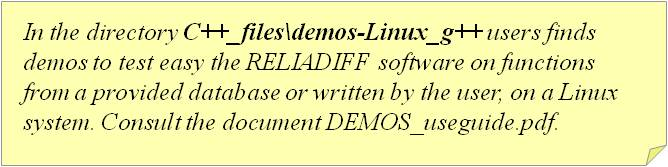
\includegraphics[scale=0.8]{rel10}
\end{flushright}
\end{figure}


\section{Content of the directory C++$\_$files/src}

The package directory is C++$\_$files/src and it contains the following files:

\begin{description}
\item  {\bf {\tt RELIADIFF.c}} 	 	 main routine for the inversion.
\item {\bf {\tt phi.c	}} 	containing the routines needed to compute the $Phi$ function \cite{RELART}.
\item {\bf {\tt RELIADIFF.h}}	 		containing some header inclusions ($stdio$, $math$, $tadiff\ldots$), a constant
definition and the prototypes of the function defined in {\tt phi.c} and {\tt RELIADIFF.c}.
\item {\bf {\tt fadbad}}  			a directory containing the software {\tt FADBAD/TADIFF} headers (authors Ole
Stauning and Claus Bendtsen \cite{2}), used to implement the Algorithmic Differentiation.
\item
{\bf {\tt Makefile}}   		to create a library to link to when compiling an application calling RELIADIFF (on a Linux system).
 \begin{itemize}
\item The command {\bf {\tt make}} creates the library {\tt libreliadiff.a}
\item The command {\bf {\tt make clean}} deletes the {\tt libreliadiff.a} file
\end{itemize}
\item {\bf {\tt SimpleCallingProgramExample.c}} 	containing a simple example of calling program for the RELIADIFF routine.
\item
{\bf  {\tt CallingProgramExecution-Linux$\_$g++}} 	a directory containing a shell script to compile and execute the provided example of calling program, on a Linux system with a g++ compiler.
 \begin{itemize}
\item
{\bf {\tt compiling$\_$a$\_$CallingProgram.sh}} 	script containing an example of how to compile and execute a C/C$\#$/C++ code using the RELIADIFF routine.
\end{itemize}
\item {\bf  {\tt CallingProgramExecution-Windows$\_$DevC++5}}  	a directory containing a DEV-C++ project to compile and execute the provided example of calling program, on a Windows system with {\em Bloodshed DEV-C++ IDE v. 4.9.9.2} installed. \begin{itemize}
\item
{\bf {\tt ExampleCallingRELIADIFFproject.dev}}	dev-project containing an example of how to compile and execute a C/C$\#$/C++ code using the RELIADIFF routine. Option given to the project:
\begin{itemize}
\item {\bf Type}: Win32 console
\item {\bf Executable Output Directory}: \begin{verbatim} ..\CallingProgramExecution-Windows_DevC++5 \end{verbatim}
\item {\bf Object File Output Directory}: \begin{verbatim} ..\CallingProgramExecution-Windows_DevC++5 \end{verbatim}
\end{itemize}
\end{itemize}

\end{description}


\newpage

\begin{thebibliography}{10}

\bibitem{RELART}  	 A. Murli, L. D'Amore, V. Mele, R. Campagna, \emph{ReLIADiff. A C++ Software Package For Real Laplace
transform Inversion based on Algorithmic Differentiation}, ACM Transactions on Mathematical Software,
0, 0, Article 0 ( 0000), 20 pages.

\bibitem{2} 	C. Bendtsen, O. Stauning, \emph{ Tadiff, a flexible C++ package for Automatic Differentiation using Taylor series expansion}, technical report IMM-REP-1997-07, Department of Mathematical Modelling, Technical University of Denmark, 2800 Lyngby, Denmark, 1997.

\end{thebibliography}



\end{document}



